\section{模型压缩}
\label{sec:compression}

LLM 的超大参数规模与计算开销给实际部署带来巨大压力，尤其在资源受限场景中更为突出。
最直接的缓解路径是模型压缩。
本节系统回顾 LLM 的网络压缩方法，覆盖量化、剪枝、知识蒸馏、低秩分解等主流技术。
在各小节中，我们结合 LLM-Viewer 对压缩对推理的影响进行分析，并给出部署建议。

\subsection{量化}
\label{sec:quantization}

在 LLM 压缩中，量化是降低存储与计算成本的核心技术。
其基本思想是将原始浮点参数映射为整数或离散表示，从而显著减少存储与计算复杂度~\citep{gholami2022survey}。
尽管量化会引入一定精度损失，但合理设计可在较小精度代价下获得明显压缩收益。

LLM 量化大体可分两类：
(1) 用于压缩预训练模型的量化；
(2) 参数高效微调量化（Q-PEFT）。
前者又可分为 QAT 与 PTQ：
QAT 在训练或再训练阶段引入量化，使模型适配低比特表示；
PTQ 在训练后直接量化，无需再训练，流程更简洁。

\subsubsection{LLM-Viewer 用例：量化的 Roofline 分析}

这里给出如何用 LLM-Viewer（Sec.~\ref{sec:llmviewer}）分析量化部署瓶颈。
在 LLM 中，关键张量包括权重、激活（含临时激活）与 KV cache：
(1) 权重必须常驻内存。例如 Llama-13b~\citep{touvron2023llama1} 在 FP16 下约占 26GB；
(2) 临时激活在推理中产生，例如各层输入在残差加法前需要保留；
(3) 自回归模型还需缓存 key/value 以支撑后续 token 生成。
我们从计算、内存占用、内存访问三方面分析量化影响。

\begin{figure}[t]
    \centering
    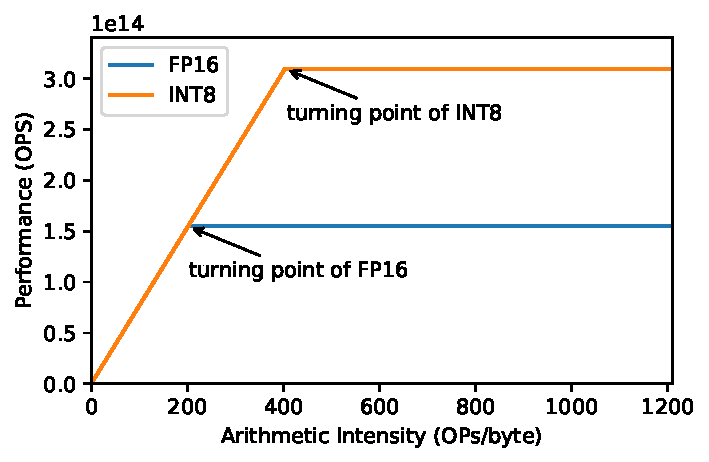
\includegraphics[width=0.95\linewidth]{ims/quantization_roofline_model.pdf}
    \caption{Nvidia A6000 在不同计算数据类型下的 Roofline 示意。}
    \label{fig:quantization_roofline_model}
\end{figure}

\begin{figure}[t]
    \centering
    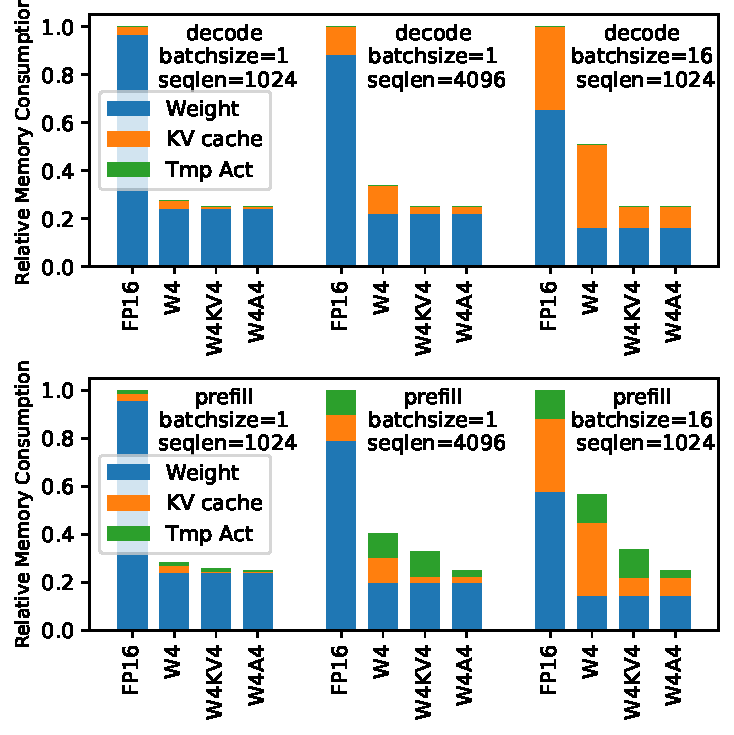
\includegraphics[width=0.95\linewidth]{ims/quantization_memory_consumption.pdf}
    \caption{Llama-2-13b 在不同量化设置下的相对内存占用。Tmp Act 表示临时激活。}
    \label{fig:quantization_memory_consumption}
\end{figure}

\textbf{计算视角：}
现代硬件（如 NVIDIA GPU）通常支持 FP32/FP16/INT8，且低比特往往有更高算力。
例如 A6000 的 FP16 与 INT8 峰值大致为 155TOP/s 与 310TOP/s。
在 Roofline 中，启用低比特计算会抬高 compute roof，对 compute-bound 层有利（图~\ref{fig:quantization_roofline_model}）。
但若仅权重量化为 INT8、激活仍是 FP16，则难以直接利用 INT8 计算单元，往往需要类型转换。
同理，当量化比特不受硬件原生支持（如 H100 不支持 INT4 计算）时，也需转换到更高比特执行。

\textbf{内存占用视角：}
不同张量量化带来的内存收益不同（图~\ref{fig:quantization_memory_consumption}）\footnote{W4：仅权重 4bit，激活 FP16；W4A4：权重与激活均 4bit；W4KV4：权重与 KV cache 量化，临时激活仍 FP16。}。
临时激活（特别是 decode 阶段）生命周期短、可快速释放，占比通常较小。
而 KV cache 会在完整回答生成结束前持续保留，且随 batch 与序列长度增大而显著增长。

\textbf{内存访问视角：}
量化可减少同等计算下的数据搬运字节数，提升算术强度，通常对应三种情况：
(1) 量化前后均 memory-bound：访存压力下降，理论性能提升（对 decode 帮助最大）；
(2) 从 memory-bound 进入 compute-bound：性能同样提升；
(3) 量化前后均 compute-bound：性能提升有限。

图~\ref{fig:quantization_memory_access_batch} 显示：小 batch 下网络前后均 memory-bound，量化可显著降时延；大 batch 下网络已趋于 compute-bound，将权重从 4bit 继续压到 2/1bit 不再明显降时延。
图~\ref{fig:quantization_memory_access_seq_len} 显示：prefill 在短序列时更易 memory-bound，量化有效；序列变长后趋向 compute-bound，收益下降。

\begin{figure}[t]
    \centering
    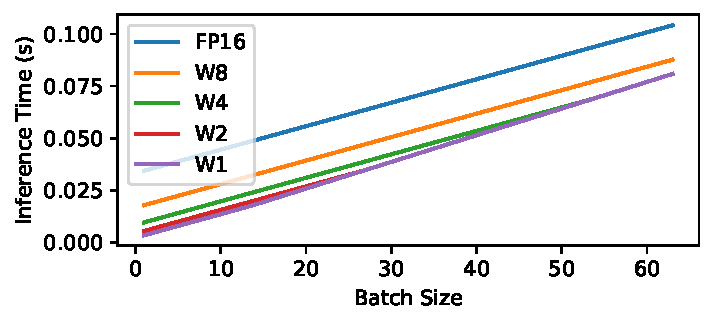
\includegraphics[width=0.95\linewidth]{ims/quantization_memory_access_batch.pdf}
    \caption{Llama-2-13b decode 阶段在不同量化设置下的推理时间（序列长=1024）。}
    \label{fig:quantization_memory_access_batch}
\end{figure}

\begin{figure}[t]
    \centering
    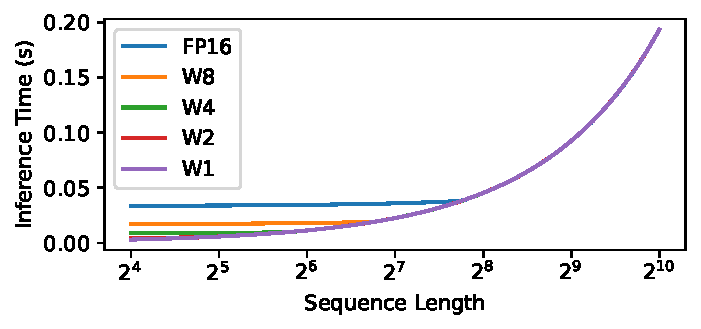
\includegraphics[width=0.95\linewidth]{ims/quantization_memory_access_seq_len.pdf}
    \caption{Llama-2-13b prefill 阶段在不同量化设置下的推理时间（batch=1）。}
    \label{fig:quantization_memory_access_seq_len}
\end{figure}

\subsubsection{用于压缩预训练 LLM 的量化}

\textbf{QAT：}
QAT~\citep{courbariaux2015binaryconnect,choi2018pact,dong2019hawq}将量化直接纳入训练过程，使模型适配低精度表示。
LLM-QAT~\citep{liu2023llm} 通过数据无关蒸馏缓解训练数据构建问题，并将量化扩展到 KV cache，在吞吐与长序列支持上带来收益。
在更低比特场景，\cite{kim2023token} 提出 TSLD 支持三值 QAT；\cite{shang2024pb} 的 PB-LLM 通过“部分二值化”保护关键权重，维持重度量化下推理能力。

\begin{figure*}[t]
    \centering
    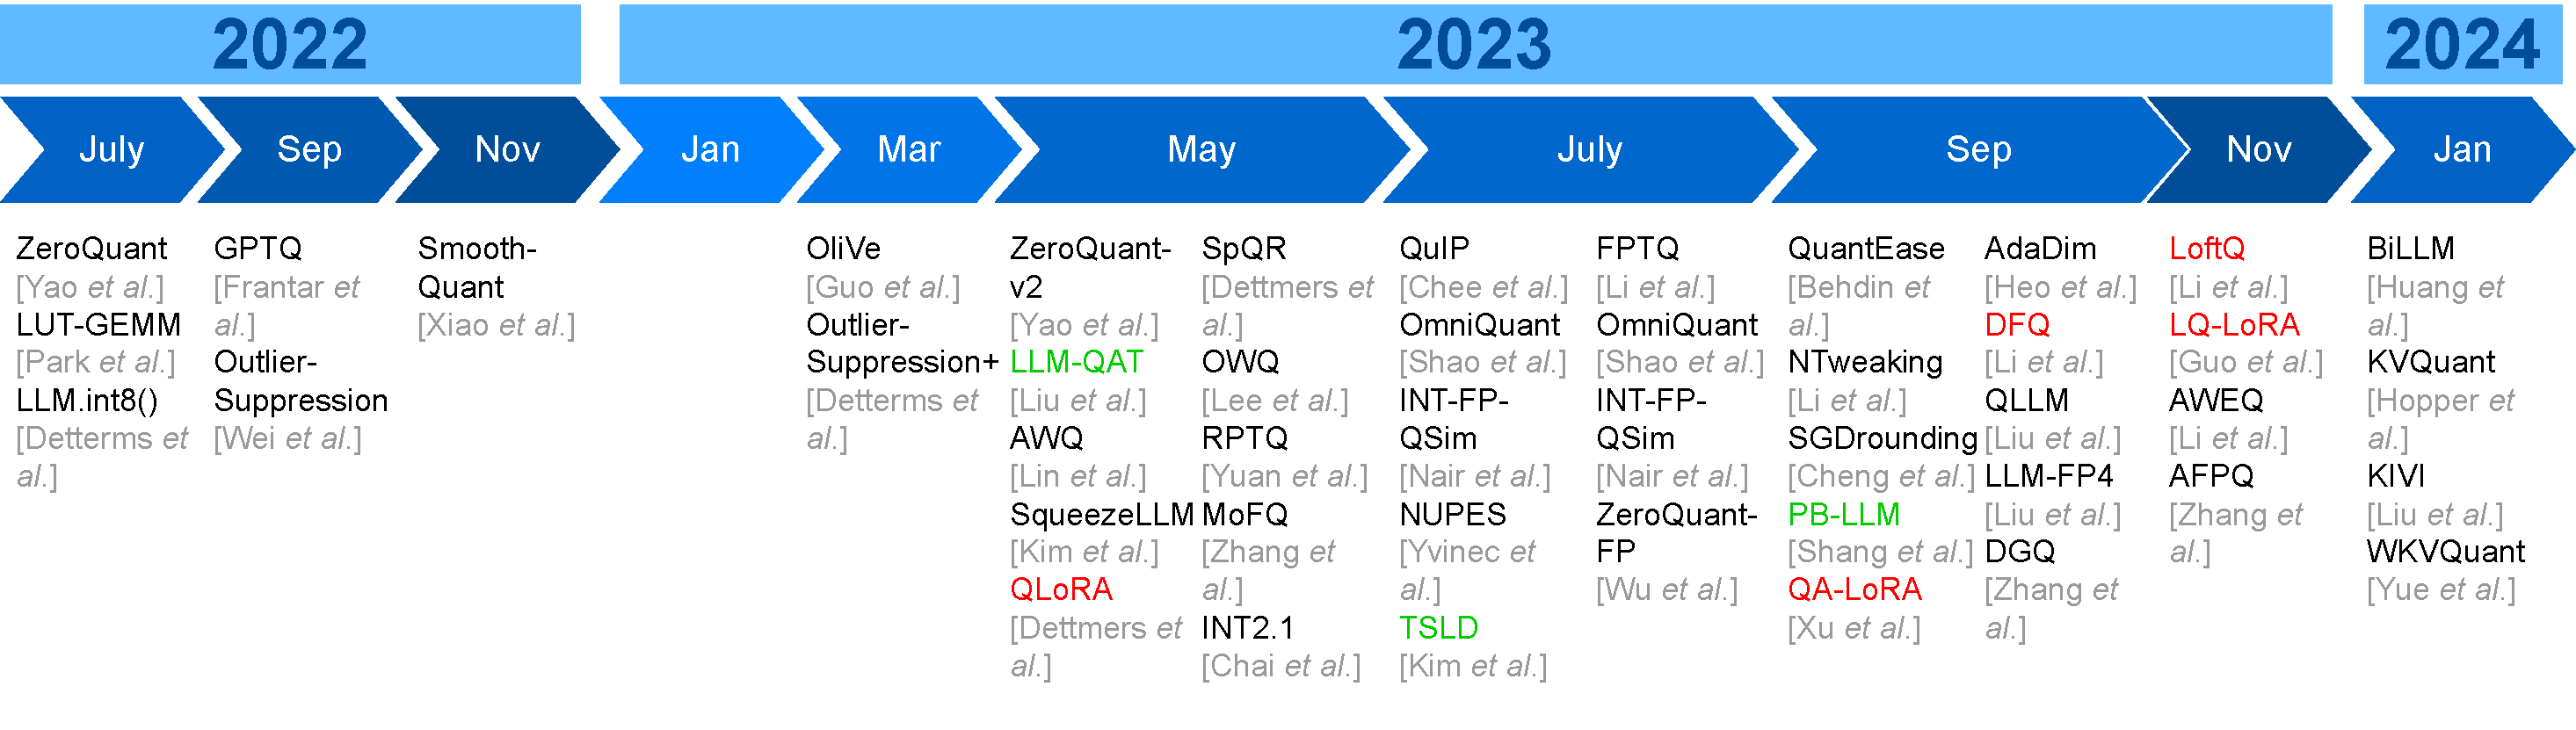
\includegraphics[width=0.99\linewidth]{ims/quantization-timeline-2024feb.pdf}
    \vspace{-0.1in}
    \caption{2022--2024 年 LLM 量化方法时间线。\textcolor{red}{红色}为 Q-PEFT，\textcolor{green}{绿色}为 QAT，其他为 PTQ。}
    \label{fig:ptq-timeline}
\end{figure*}

\noindent\textbf{PTQ：}
PTQ 在训练后量化参数，不改架构且无需再训练，实施简单，尤其适合超大模型。
在 LLM 场景中，QAT 成本往往过高，因此 PTQ 具有较高实践价值。

PTQ 中大量工作聚焦 \textbf{仅权重量化}：
LUT-GEMM~\citep{park2023lut}、LLM.int8()~\citep{dettmers2022llm}、ZeroQuant~\citep{yao2022zeroquant}、GPTQ~\citep{frantar2022gptq}、AWQ~\citep{lin2023awq, kim2023squeezellm}、OWQ~\citep{lee2023owq}、SpQR~\citep{dettmers2023spqr}、QuantEase~\citep{behdin2023quantease} 等，重点在降低比特并抑制精度损失。
更低比特方面，QuIP~\citep{chee2023quip}、Norm Tweaking~\cite{li2023norm}、PB-LLM~\citep{shang2024pb}、BiLLM~\citep{huang2024billm} 等推动到 2bit 甚至接近 1bit。

另一类 PTQ 关注 \textbf{权重+激活量化}：
SmoothQuant~\citep{xiao2023smoothquant}、RPTQ~\citep{yuan2023rptq}、OliVe~\citep{guo2023olive}、ZeroQuant-FP~\citep{wu2023zeroquant}、FPTQ~\cite{li2023fptq} 等，主要处理激活离群值、通道差异与硬件友好映射。

\begin{figure}[t]
    \centering
    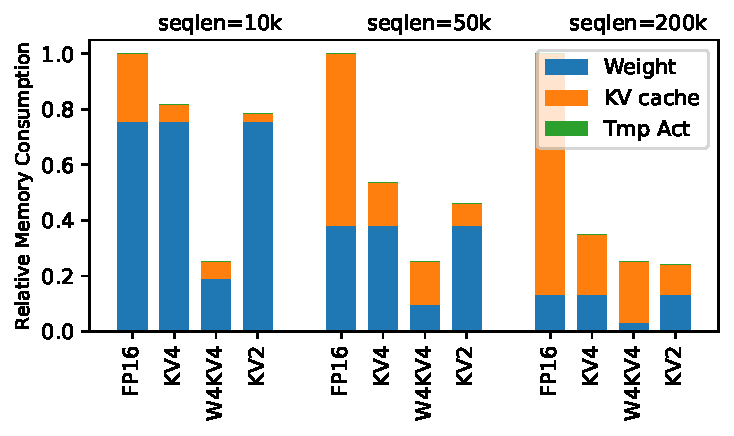
\includegraphics[width=0.95\linewidth]{ims/quantization_memory_consumption_long_seq.pdf}
    \caption{Llama-2-13b decode 阶段在不同量化设置下的内存占用（batch=1）。}
    \label{fig:quantization_memory_consumption_long_seq}
\end{figure}

自 2023 年底以来，长上下文快速增长，KV cache 成为关键内存瓶颈。
例如 Gemini 1.5~\citep{gemini2024} 在生产中可处理百万 token；文档/图像/视频场景也常需万级 token。
因此 \textbf{KV Cache 量化} 变得尤为重要。
2024 年已有多项工作推进该方向，如 \cite{hooper2024kvquant}、KIVI~\citep{liu2024kivi}、WKVQuant~\cite{yue2024wkvquant}。
图~\ref{fig:quantization_memory_consumption_long_seq} 显示，当序列长度超过 50k，KV cache 占据大部分内存，其量化可显著降低总内存。

\subsubsection{参数高效微调量化（Q-PEFT）}

PEFT 是 LLM 重要方向，其中 LoRA~\citep{hu2021lora,valipour2022dylora} 通过低秩分解适配器显著减少可训练参数，效果接近全量微调，详见综述~\citep{hu2023llm}。

Q-PEFT 将量化融入 PEFT 流程，形成新的效率范式。
代表工作包括 PEQA~\citep{kim2023memory}、DFT~\citep{li2023qft}、QLoRA~\citep{dettmers2023qlora}。
QLoRA 通过新数据类型、双重量化、paged optimizer 等机制显著省内存，并实现单卡大模型微调。

QLoRA 的限制在于通常难以稳定到 4bit 以下。
为此，LQ-LoRA~\citep{guo2023lq}、Loft-Q~\citep{li2023loftq}、QA-LoRA~\citep{xu2023qa} 等工作进一步探索低比特微调，提升泛化并减少 PTQ 常见精度损失。

\subsubsection{LLM 量化讨论}
图~\ref{fig:ptq-timeline} 展示了量化技术演进：从 PTQ 主导，逐步过渡到 QAT 与 Q-PEFT 并行发展。
这反映了社区针对 PTQ 性能瓶颈的适应性转向，也表明 QAT/Q-PEFT 正成为高效 LLM 推理的重要增长点。

\subsection{剪枝}

剪枝~\citep{lecun1989optimal,liang2021pruning}通过删除冗余参数压缩模型，是另一类主流方法。
在 LLM 中，参数占据主要体量与计算开销，因此合理剪枝可在较小性能损失下提升效率。
剪枝大致分为非结构化与结构化两类。

\subsubsection{非结构化剪枝}
非结构化剪枝按权重/神经元粒度删除，通常精度保持较好，但稀疏模式不规则，对软件/硬件支持要求高。
SparseGPT~\citep{frantar2023sparsegpt} 将问题转化为大规模稀疏回归，单 GPU 数小时可处理 175B 模型，并在高稀疏率下保持较好性能。
Wanda~\cite{sun2023simple} 通过权重幅值与输入范数评估重要性，显著降低重构开销。
\cite{yin2023outlier} 通过非均匀分层稀疏率重点处理离群层。
Flash-LLM~\citep{xia2023flash} 则从硬件侧提出稀疏加载+稠密计算以利用 Tensor Core。

\subsubsection{结构化剪枝}
结构化剪枝删除整层或整块结构，规则性好、硬件友好，但对性能影响通常更明显。
LLM-Pruner~\citep{ma2023llm} 使用一次性结构化剪枝并结合 LoRA 恢复；
Sheared Llama~\citep{xia2023sheared} 结合目标架构裁剪与动态批加载；
Compresso~\citep{guo2023compresso} 通过协同学习将 Llama-7B 剪至 5.4B 并维持性能。

\subsection{知识蒸馏}

知识蒸馏~\citep{hinton2015distilling,gou2021knowledge} 将大模型（teacher）能力迁移给小模型（student），在降低资源消耗的同时保持任务能力~\citep{gou2021knowledge,shang2021lipschitz}。
LLM 蒸馏常分为白盒与黑盒两类，详细综述可见~\citep{xu2024kdsurvey}。

\subsubsection{白盒蒸馏}
白盒蒸馏可访问 teacher 架构与权重，student 除学习输出外还能学习中间表示与决策过程。
MiniLLM~\citep{gu2023knowledge}、GKD~\citep{agarwal2023gkd}、Homotopic Distillation~\citep{liang2023homodistil}、\cite{liang2023less}、AD-KD~\citep{wu2023ad} 等从损失函数、训练稳定性、层级匹配与可解释归因迁移等角度提升蒸馏质量。

\subsubsection{黑盒蒸馏}
黑盒蒸馏不依赖 teacher 内部信息，仅通过输入-输出行为迁移能力。
Multitask-ICT~\citep{huang2022context}、LaMini-LM~\citep{wu2023lamini}、PromptMix~\cite{sahu2023promptmix}、Lion~\citep{jiang2023lion} 等是代表性方法。

黑盒蒸馏也常用于迁移 CoT 推理能力。
例如 \cite{fu2023specializing}、SCOTT~\citep{wang2023scott}、Distilling step-by-step~\citep{hsieh2023distilling}、\cite{li2023symbolic}、\cite{chae2023dialogue} 等，分别从对比解码监督、多任务蒸馏、符号化 CoT 与对话场景推理蒸馏等角度推进该方向。

\subsection{分解（Factorization）}

低秩分解~\citep{kishore2017literature} 是压缩 DNN 的经典方法，近年在大模型压缩与加速中持续发展~\citep{schotthofer2022low}。

ASVD~\citep{yuan2023asvd} 是将分解用于 LLM 压缩的早期代表工作之一，通过激活感知处理离群值并进行分层校准，提高分解精度与效率。
LASER~\citep{sharma2023truth} 发现选择性移除高阶分量可在若干场景提升模型表现。
TensorGPT~\citep{xu2023tensorgpt} 则面向 embedding 层，通过 Tensor-Train Decomposition（TTD）~\citep{oseledets2011tensor} 以低秩张量形式存储大规模 embedding。
